
\documentclass[14pt]{beamer}

\usepackage{color}
\usepackage{tikz}

\usetheme{Warsaw}
\begin{document}

\title{Simulation of a particle detector}
\author{Arnaud Schils \\ Simon Lardinois}
\maketitle

\begin{frame}
\frametitle{Summary}

\begin{enumerate}
  \setlength\itemsep{1.4em}
  \item Particle detector physics
  \item Computing the \textcolor{red}{potential} in the detector
  \item Computing the \textcolor{red}{current} induced by a particle
  \item Conclusion
\end{enumerate}
\end{frame}

\begin{frame}

\frametitle{Particle detector physics}
\framesubtitle{The detector}

\begin{figure}[H]
\begin{center}
	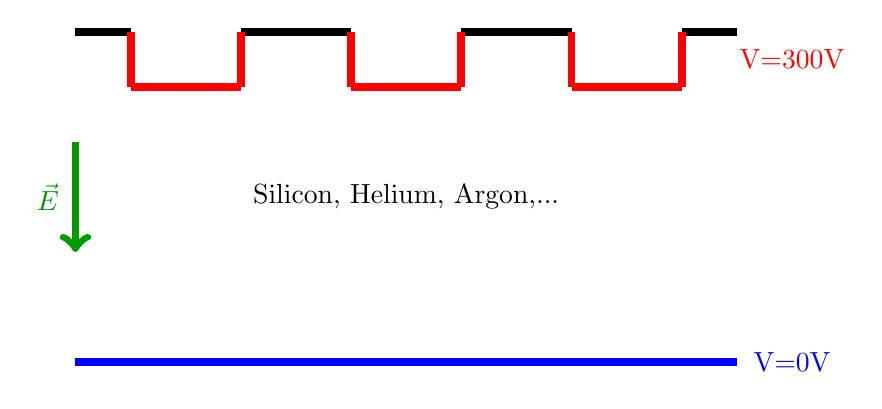
\begin{tikzpicture}[scale=0.7]
    \draw[line width=1mm, black] (-6,3) -- (-5,3);
    \draw[line width=1mm, black] (-3,3) -- (-1,3);
    \draw[line width=1mm, black] (1,3) -- (3,3);
    \draw[line width=1mm, black] (5,3) -- (6,3);

    \draw[line width=1mm, red] (-5,2) -- (-3,2);
    \draw[line width=1mm, red] (-1,2) -- (1,2);
    \draw[line width=1mm, red] (3,2) -- (5,2);

    \draw[line width=1mm, red] (-5,3) -- (-5,2);
    \draw[line width=1mm, red] (-3,3) -- (-3,2);

    \draw[line width=1mm, red] (-1,3) -- (-1,2);
    \draw[line width=1mm, red] (1,3) -- (1,2);

    \draw[line width=1mm, red] (3,3) -- (3,2);
    \draw[line width=1mm, red] (5,3) -- (5,2);

    \draw[line width=1mm, blue] (-6,-3) -- (6,-3);
    \node[blue] at (7,-3) {V=0V};
    \node[red] at (7,2.5) {V=300V};
    \node at (0,0) {Silicon, Helium, Argon,...};

    \node[black!40!green] at (-6.5,0) {$\vec{\text{E}}$};
    \draw[line width=1mm, black!40!green, ->] (-6, 1) -- (-6,-1);


	\end{tikzpicture}
\end{center}
\end{figure}




\end{frame}

\end{document}
